\documentclass[eng,openany]{mgr}
\usepackage{listings}
\usepackage[english]{babel}
\usepackage{graphicx}
\usepackage{hyperref}
\usepackage{tabularx,colortbl} 
\usepackage{rotating}
\usepackage[utf8]{inputenc} 
\setlength\parindent{24pt}
\usepackage[parfill]{parskip}
\usepackage[table,kernelfbox,hyperref]{xcolor}
\usepackage{fancyhdr}
\usepackage{gauss}
%\usepackage[colorinlistoftodos]{todonotes}

\hypersetup{colorlinks=true}
\hypersetup{xurlbordercolor=red!70!black}
\hypersetup{xlinkbordercolor=blue!70!black}
\hypersetup{linkcolor=blue!60!black}
\hypersetup{urlcolor=red!50!black}
\hypersetup{citecolor=green!30!black}
\rfoot{Page \thepage}
\renewcommand\lstlistlistingname{List of Listings}
\newcommand{\linia}{\rule{\linewidth}{0.4mm}}

\definecolor{listlightgray}{gray}{0.93}

\newcommand{\lstsetmylst} {
\lstset{frame = tb,
breaklines=true,
framerule = 0.25pt,
float,
fontadjust,
backgroundcolor={\color{listlightgray}},
basicstyle = {\ttfamily\footnotesize},
identifierstyle = {\ttfamily},
stringstyle = {\ttfamily},
showstringspaces = false,
showtabs = false,
numbers = left,
numbersep = 6pt,
tabsize = 4,
language=C,
floatplacement=!h
}
}

\newcommand{\lstsetatc} {
\lstset{frame = tb,
breaklines=true,
framerule = 0.25pt,
float,
fontadjust,
backgroundcolor={\color{listlightgray}},
basicstyle = {\ttfamily\footnotesize},
keywordstyle = {\ttfamily\color{listkeyword}\textbf},
identifierstyle = {\ttfamily},
commentstyle = {\ttfamily\color{listcomment}\textit},
stringstyle = {\ttfamily},
showstringspaces = false,
showtabs = false,
numbers = left,
numbersep = 6pt,
numberstyle={\ttfamily\color{listnumbers}},
tabsize = 4,
language=C,
floatplacement=!h
}
}

\newcommand{\lstsetatbashnum} {
\lstset{frame = tb,
breaklines=true,
framerule = 0.25pt,
aboveskip=2ex,
float,
fontadjust,
backgroundcolor={\color{listlightgray}},
basicstyle = {\ttfamily\footnotesize},
keywordstyle = {\ttfamily\color{listkeyword}\textbf},
identifierstyle = {\ttfamily},
commentstyle = {\ttfamily\color{listcomment}\textit},
stringstyle = {\ttfamily},
showstringspaces = false,
showtabs = false,
numbers = left,
numbersep = 6pt,
numberstyle={\ttfamily\color{listnumbers}},
tabsize = 4,
language=bash,
floatplacement=!h
}
}
\lstsetmylst
\author{Jaroslaw M. Szumega}
\title{}
\engtitle{}
\supervisor{Rafal Zdunek, D.Sc, K-4/W4}
\field{Electronics}
\specialisation{Advanced Applied Electronics}
\date{21.03.2017}
\begin{document}
\selectlanguage{english}
\maketitle
\tableofcontents
\newpage

\chapter{Solution to the given problems}
(Problems 1, 3, 4 and 7 are solved analytically, without using any of selected algorithms. Result are checked with built-in Octave/Matlab function.)

\textbf{Problem 1} - Compute the eigenpairs of the matrices. Verify that trace equals to eigenvalues sum and the determinant to their product. Which matrix is singular?

To find eigenvalues, the following calculations will be used:\\
\begin{math}
Ax - \lambda x = 0 \\
(A - \lambda I) x = 0 \\
det(A - \lambda I) = 0
\end{math}
Then the characteristic polynomial can be determined. It's roots are the eigenvalues.

\textbf{Matrix A1}

\[
A_1 =
\begin{bmatrix}
1 & 0 & 0  \\
2 & 1 & 0 \\
0 & 0 & 3 
\end{bmatrix}
\]

\[
det
\begin{bmatrix}
1 -\lambda & 0 & 0  \\
2 & 1-\lambda & 0 \\
0 & 0 & 3-\lambda 
\end{bmatrix}
=(1-\lambda)(1-\lambda)(3-\lambda)
\]

\begin{math}
For \lambda = 1:\\
\begin{bmatrix}
0 & 0 & 0  \\
2 & 0 & 0 \\
0 & 0 & 2 
\end{bmatrix}
\begin{bmatrix}
x_1 \\
x_2 \\
x_3
\end{bmatrix}
= 0\; =>
\begin{matrix}
2x_1 = 0\\
2x_3 = 0\\
(no\;x_2\;formula)
\end{matrix}
=>
x = 
\begin{bmatrix}
0\\
t \\
0
\end{bmatrix}
\end{math}

\begin{math}
For \lambda = 3:\\
\begin{bmatrix}
-2 & 0 & 0  \\
2 & -2 & 0 \\
0 & 0 & 0 
\end{bmatrix}
\begin{bmatrix}
x_1 \\
x_2 \\
x_3
\end{bmatrix}
= 0\; =>
\begin{matrix}
-2x_1 = 0\\
2x_1 -2x_2 = 0\\
(no\;x_3\;formula)
\end{matrix}
=>
x = 
\begin{bmatrix}
0\\
0 \\
t
\end{bmatrix}
\end{math}
\\ \\ 
$tr(A) = 1 + 1 + 3 = 5$\\
$\sum \lambda = 1 + 1 + 3 = 5
\\ \\
det(A) = 1 \cdot 1 \cdot 3$ = 3\\
$\prod \lambda = 1 \cdot 1 \cdot 3$ = 3
\\
Matrix determinant is non--zero, so the matrix is not singular.
\newpage
\textbf{Matrix A2}
\[
A_2 =
\begin{bmatrix}
	0 & -2 & 1  \\
	1 & 3 & -1 \\
	0 & 0 & 1 
\end{bmatrix}
\]

\[
det
\begin{bmatrix}
0-\lambda & -2 & 1  \\
1 & 3-\lambda & -1 \\
0 & 0 & 1-\lambda 
\end{bmatrix}
= (Sarrus\;theorem =>)(1-\lambda)(1-\lambda)(3-\lambda) = \\ 
\]
\[
= (-\lambda)(3-\lambda)(1-\lambda) - (-2)(1-\lambda) = (1-\lambda)(\lambda ^2 - 3\lambda + 2)
\]

\begin{math}
For \lambda = 1:\\
\begin{bmatrix}
-1 & -2 & 1  \\
1 & 2 & -1 \\
0 & 0 & 0 
\end{bmatrix}
\begin{bmatrix}
x_1 \\
x_2 \\
x_3
\end{bmatrix}
= 0\; =>
\begin{matrix}
-x_1 -2x_2+x_3 = 0\\
x_1+2x_2-x_3 = 0\\

\end{matrix}
=>
x = 
\begin{bmatrix}
-2v_2+v_3\\
v_2 \\
v_3
\end{bmatrix}
\end{math}

\begin{math}
For \lambda = 2:\\
\begin{bmatrix}
-2 & -2 & 1  \\
1 & 1 & -1 \\
0 & 0 & -1 
\end{bmatrix}
\begin{bmatrix}
x_1 \\
x_2 \\
x_3
\end{bmatrix}
= 0\; =>
\begin{matrix}
-2x_1 -2x_2+x_3 = 0\\
x_1+x_2-x_3 = 0\\
(-x_3=0)
\end{matrix}
=>
x = 
\begin{bmatrix}
v\\
-v \\
0
\end{bmatrix}
\end{math}
\\ \\ 
$tr(A) = 3 +1 = 4$\\
$\sum \lambda = 1+1+2 = 4
\\ \\
det(A) = 2\\
\prod \lambda = 1 \cdot 1 \cdot 2$ = 2
\\
Matrix determinant is non--zero, so the matrix is not singular.
\\
\\
\textbf{Matrix A3}
\[
A_3 =
\begin{bmatrix}
	4 & 1 & 0  \\
	1 & 4 & 1 \\
	0 & 1 & 4 
\end{bmatrix}
\]

\[
de
A_3 =
\begin{bmatrix}
4-\lambda & 1 & 0  \\
1 & 4-\lambda & 1 \\
0 & 1 & 4-\lambda 
\end{bmatrix}t
= (Sarrus\;theorem =>)(4-\lambda)(4-\lambda)(4-\lambda)- (4-\lambda) - (4-\lambda) = 
\]
\[
= (4-\lambda)(\lambda^2 - 8 \lambda + 14) = (4-\lambda)(\lambda - (4+\sqrt{2}))(\lambda - (4-\sqrt{2}))
\]

\begin{math}
For \lambda = 4:\\
\begin{bmatrix}
0 & 1 & 0  \\
1 & 0 & 1 \\
0 & 1 & 0 
\end{bmatrix}
\begin{bmatrix}
x_1 \\
x_2 \\
x_3
\end{bmatrix}
= 0\; =>
\begin{matrix}
-x_1 -2x_2+x_3 = 0\\
x_1+2x_2-x_3 = 0\\

\end{matrix}
=>
x = 
\begin{bmatrix}
-2v_2+v_3\\
v_2 \\
v_3
\end{bmatrix}
\end{math}

\begin{math}
For \lambda = 4+\sqrt{2}:\\
\begin{bmatrix}
-\sqrt{2} & 1 & 0  \\
1 & -\sqrt{2} & -1 \\
0 & 1 & -\sqrt{2} 
\end{bmatrix}
\begin{bmatrix}
x_1 \\
x_2 \\
x_3
\end{bmatrix}
= 0\; =>
\begin{matrix}
-\sqrt2x_1 +x_2 = 0\\
x_1-\sqrt2x_2+x_3 = 0\\
x_2-\sqrt2x_3=0
\end{matrix}
=>
x = 
\begin{bmatrix}
v\\
\sqrt2v \\
v
\end{bmatrix}
\end{math}

\begin{math}
For \lambda = 4-\sqrt{2}:\\
\begin{bmatrix}
\sqrt{2} & 1 & 0  \\
1 & \sqrt{2} & -1 \\
0 & 1 & \sqrt{2} 
\end{bmatrix}
\begin{bmatrix}
x_1 \\
x_2 \\
x_3
\end{bmatrix}
= 0\; =>
\begin{matrix}
\sqrt2x_1 +x_2 = 0\\
x_1+\sqrt2x_2+x_3 = 0\\
x_2+\sqrt2x_3=0
\end{matrix}
=>
x = 
\begin{bmatrix}
v\\
-\sqrt2v \\
v
\end{bmatrix}
\end{math}
\\ \\ 
$tr(A) = 4+4+4 = 12$\\
$\sum \lambda = 4 + 4 + \sqrt2 + 4 - \sqrt2 = 12
\\ \\
det(A) = 56\\
\prod \lambda = 4 \cdot (4+\sqrt2) \cdot (4+\sqrt2) = 4 \cdot (4^2-(\sqrt2)^2)= 4 \cdot 14 = 56$
\\
Matrix determinant is non--zero, so the matrix is not singular.

\textbf{Matrix A4}
\[
A_4 =
\begin{bmatrix}
1 & 2 & 3 & 4\\
5 & 6 & 7 & 8\\
9 & 10 & 11 & 12\\
13 & 14 & 15 & 16
\end{bmatrix}
\begin{matrix}
R2-2R1 \\
R3-R1\\
=\\
R4-4R1\\
&
\end{matrix}
\begin{bmatrix}
1 & 2 & 3 & 4\\
3 & 2 & 1 & 0\\
6 & 4 & 2 & 0\\
9 & 6 & 3 & 0
\end{bmatrix}
\begin{matrix}
 \\
R3-2R2\\
=\\
R4-3R2\\
&
\end{matrix}
\begin{bmatrix}
1 & 2 & 3 & 4\\
3 & 2 & 1 & 0\\
0 & 0 & 0 & 0\\
0 & 0 & 0 & 0
\end{bmatrix}
\]
det(A) = 0, so matrix is singular.
\\
\\
Now calculating the eigenvalues:\[
\begin{bmatrix}
1-\lambda & 2 & 3 & 4\\
5 & 6-\lambda & 7 & 8\\
9 & 10 & 11-\lambda & 12\\
13 & 14 & 15 & 16-\lambda
\end{bmatrix}
=>
\begin{matrix}
& \lambda_1 = 0\\
& \lambda_2 = 0\\
& \lambda_3 = 17+3\sqrt{41}\\
&\lambda_4 = 17-3\sqrt{41}\\
\end{matrix}
\]
\\ \\ 
$tr(A) = 1+6+11+16 = 34 = 12\\
\sum \lambda = 0 + 0 + 17 +3\sqrt{41}+17-3\sqrt{31} = 34
\\ \\
det(A) = 0\\
\prod \lambda = 0$
\\
Matrix determinant is zero, so the matrix is singular.
\newpage
\begin{figure}[h]
\centering
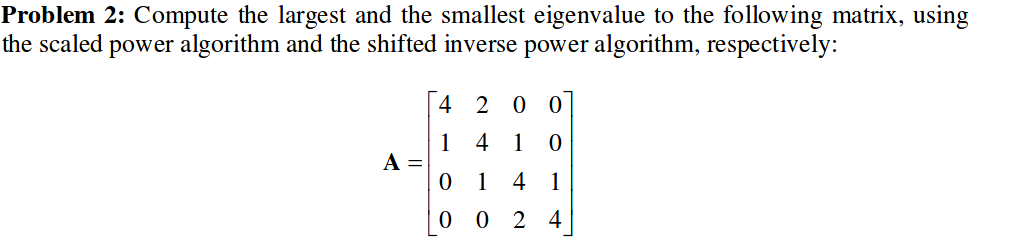
\includegraphics[width=0.8\linewidth]{screenshot001}
\label{fig:screenshot001}
\end{figure}
To compute the required values, the Scaled Power algorithm (Alg.1) and the shift inverse Power algorithm (Alg.2) were coded.

The task solution was designed in the following Octave code:
\begin{lstlisting}
A = [4 2 0 0; 1 4 1 0; 0 1 4 1; 0 0 2 4]
iterations = 10;
#computing the biggest and smallest eigenpairs

disp(['Eigenproblems using Power methods:'])

[eigenvalueMAX, eigenvectorMAX] = scaledpower(A, iterations)
[eigenvalueMIN, eigenvectorMIN] = inversepower(A, iterations)
\end{lstlisting}

That gave the results:
\begin{figure}[h]
\centering
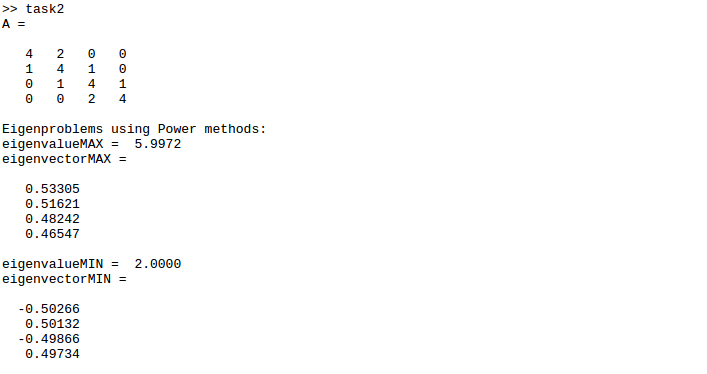
\includegraphics[width=0.8\linewidth]{screenshot002}
\label{fig:screenshot002}
\end{figure}

As it can be compared, after 10 iterations they are quite correct approximation of the exact values:
\begin{figure}[h]
\centering
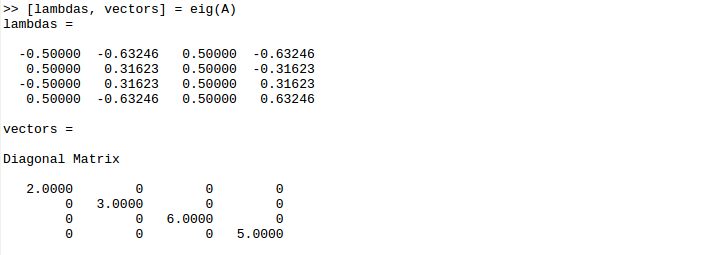
\includegraphics[width=0.8\linewidth]{screenshot003}
\label{fig:screenshot003}
\end{figure}
\newpage
\begin{figure}[h]
\centering
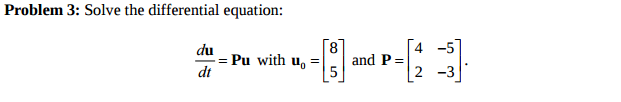
\includegraphics[width=0.8\linewidth]{screenshot004}
\label{fig:screenshot004}
\end{figure}
Solution of the differential equation has the following form:
\begin{center}
$u = \alpha \cdot exp\{\lambda t\}$\\
\end{center}
So in this particular case we are looking for:\\
$u_1 = \alpha_1 \cdot exp\{\lambda_1 t\}$\\
$u_2 = \alpha_2 \cdot exp\{\lambda_2 t\}$
\[
\begin{bmatrix}
4& -5\\
2& -3\\
\end{bmatrix}
\begin{bmatrix}
\alpha_1\\
\alpha_2\\
\end{bmatrix}
= \lambda
\begin{bmatrix}
\alpha_1\\
\alpha_2\\
\end{bmatrix}
\]

Now, we are calculating the eigenvalues:
\[
det
\begin{bmatrix}
4-\lambda&-5 \\
2& -5-\lambda\\
\end{bmatrix}
= (4-\lambda)(-3-\lambda)+10 = -12 -4\lambda +3\lambda + \lambda^2 + 10 = \lambda^2 = \lambda -2 = (\lambda-2)(\lambda+1)
\]

$For \lambda=2:$
\[
\begin{bmatrix}
2 & -5\\
2 & -5
\end{bmatrix}
\begin{bmatrix}
x_1\\
x_2
\end{bmatrix}
= 0 =>
\begin{matrix}
2x_1 - 5x_2 = 0&\\
so\; 2x_1 = 5x_2&
\end{matrix}
=> x =
\begin{bmatrix}
 5t\\
 2t
\end{bmatrix}
\]

$For \lambda=-1$:
\[
\begin{bmatrix}
5 & -5\\
2 & -2
\end{bmatrix}
\begin{bmatrix}
x_1\\
x_2
\end{bmatrix}
= 0 =>
\begin{matrix}
5x_1 = 5x_2&\\
so \; x_1 = x_2&
\end{matrix}
=> x =
\begin{bmatrix}
t\\
t
\end{bmatrix}
\]

And now the solution is in the following form:
\[
u = c_1 exp\{2t\}
\begin{bmatrix}
5\\
2
\end{bmatrix}
+ c_2 exp\{-t\}
\begin{bmatrix}
1\\
1
\end{bmatrix}
\]
Using initial condition the c values will be calculated (assuming eigenvector for t=1).
\[
\begin{bmatrix}
5 & 1\\
2 & 1
\end{bmatrix}
\begin{bmatrix}
c_1\\
c_2
\end{bmatrix}
=
\begin{bmatrix}
8\\5
\end{bmatrix}
=> 
\begin{matrix}
5c_1+c_2 = 8\\
2c_1+c_2 = 5
\end{matrix}
=>
\begin{matrix}
c_1 = 1\\
c_2 = 3
\end{matrix}
\]

Assembling all calculations, the solution to the differential equation is:
\[
u = 1\cdot exp\{2t\}
\begin{bmatrix}
5\\2
\end{bmatrix}
+
3\cdot exp\{-t\}
\begin{bmatrix}
1\\1
\end{bmatrix}
\]
\newpage
\begin{figure}[h]
\centering
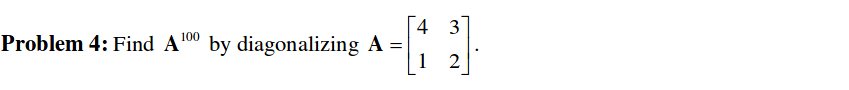
\includegraphics[width=0.8\linewidth]{screenshot005}
\label{fig:screenshot005}
\end{figure}
Matrix can be diagonalized, if it has an inverse. So at first the determinant must be non-zero.

$det(A) = 4\cdot2 - 3\cdot1 = 5$

The eigenvalues need to be calculated
\[
det
\begin{bmatrix}
4-\lambda&3\\
1 & 2-\lambda
\end{bmatrix}
= (4-\lambda)(2-\lambda)-3 = 8 - 4\lambda -2\lambda + \lambda^2 -3 = (\lambda-1)(\lambda-5)
\] 

$For \lambda=1$:
\[
\begin{bmatrix}
3 & 3\\
1 & 1
\end{bmatrix}
\begin{bmatrix}
x_1\\
x_2
\end{bmatrix}
= 0 =>
\begin{matrix}
3x_1 + 3x_2 = 0&\\
x_1 = -x_2&
\end{matrix}
=> x_1 =
\begin{bmatrix}
1\\
-1
\end{bmatrix}
\]
$For \lambda=5$:
\[
\begin{bmatrix}
-1 & 3\\
1 & -3
\end{bmatrix}
\begin{bmatrix}
x_1\\
x_2
\end{bmatrix}
= 0 =>
\begin{matrix}
-x_1 + 3x_2 = 0&\\
x_1 - 3x_2 = 0&
\end{matrix}
=> x_1 = 3x_2
=>
x_2=
\begin{bmatrix}
3\\
1
\end{bmatrix}
\]

Now to calculate $A^{100}$ we will use the following formula:\\
\[
A^{100} = X \Lambda^k X^{-1}
\]
And to calculate $\Lambda$ itself:
\[
\\
\Lambda = X^{-1}AX
\]
The matrices:\[
X = 
\begin{bmatrix}
1 &3\\
-1 & 1
\end{bmatrix}
\; \; \;\; \; \;
X^{-1} = 
\begin{bmatrix}
0.25 &-0.75\\
0.25 & 0.25
\end{bmatrix}
\; \; \;\; \; \;
\Lambda =
\begin{bmatrix}
1 &0\\
0 & 5
\end{bmatrix}
\]

And the final calculation:
\[
A^{100} = X \Lambda^{100} X^{-1} = 
\begin{bmatrix}
1 &3\\
-1 & 1
\end{bmatrix}
\begin{bmatrix}
1 &0\\
0 & 5
\end{bmatrix}
^{100}
\begin{bmatrix}
0.25 &-0.75\\
0.25 & 0.25
\end{bmatrix}
=
\begin{bmatrix}
   5.9165e+69&   5.9165e+69\\
   1.9722e+69&   1.9722e+69
\end{bmatrix}
\]
\newpage
\begin{figure}[h]
\centering
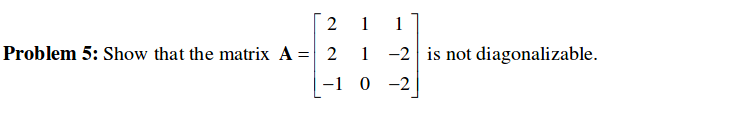
\includegraphics[width=0.8\linewidth]{screenshot006}
\label{fig:screenshot006}
\end{figure}
Matrix is diagonalizable if:
\begin{itemize}
	\item can be inverted,
	\item has n linearly independent eigenvectors,
	\item surely is diagonalizable if has n distinct eigenvalues.
\end{itemize}
\[
det
\begin{bmatrix}
2 &1 &1\\
2 &1 &-2\\
-1 &0 &-2
\end{bmatrix}
= 3
\]
Determinant is not equal to zero, so matrix has an inverse.
\\

Using coded "basic QR iteration" (Algorithm 3) we will search eigenvalues and eigenvectors.

\begin{lstlisting}
[l,v] = iterqr(A, 100000)
A =
2   1   1
2   1  -2
-1   0  -2

l =
Diagonal Matrix

3.0000	 0         0
0		-1.0000    0
0        0        -1.0000


v =
0.63500    0.40825    0.40825 
0.76200   -0.81650   -0.81650 
-0.12700  -0.40825   -0.40825
\end{lstlisting}

The calculations show, that the eigenvalues are not distinct -- there is a possibility that diagonal do not exists.\\
To be completely sure, the eigenspace has to be estimated.
Looking at the eigenvectors value, we can see that two of them are equal. Therefore they are linearly dependent.
\\

The conclusion is that the diagonal of the presented matrix does not exist.
\newpage
\begin{figure}[h]
\centering
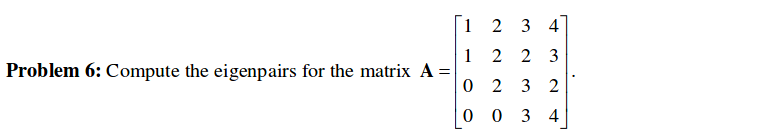
\includegraphics[width=0.8\linewidth]{screenshot007}
\label{fig:screenshot007}
\end{figure}
The following matlab code (with coded algorithms) was used to perform computations:
\begin{lstlisting}
A =    [1 2 3 4; 
		1 2 2 3; 
		0 2 3 2; 
		0 0 3 4];

disp(['Matlab embedded eig()'])
[lambda, vector] = eig(A)
disp(['QR iteration'])
[lambda, vector] = iterqr(A,100)
disp(['Single shift QR'])
[lambda, vector] = iterqr_shift(A,100)
\end{lstlisting}
\begin{figure}[h]
\centering
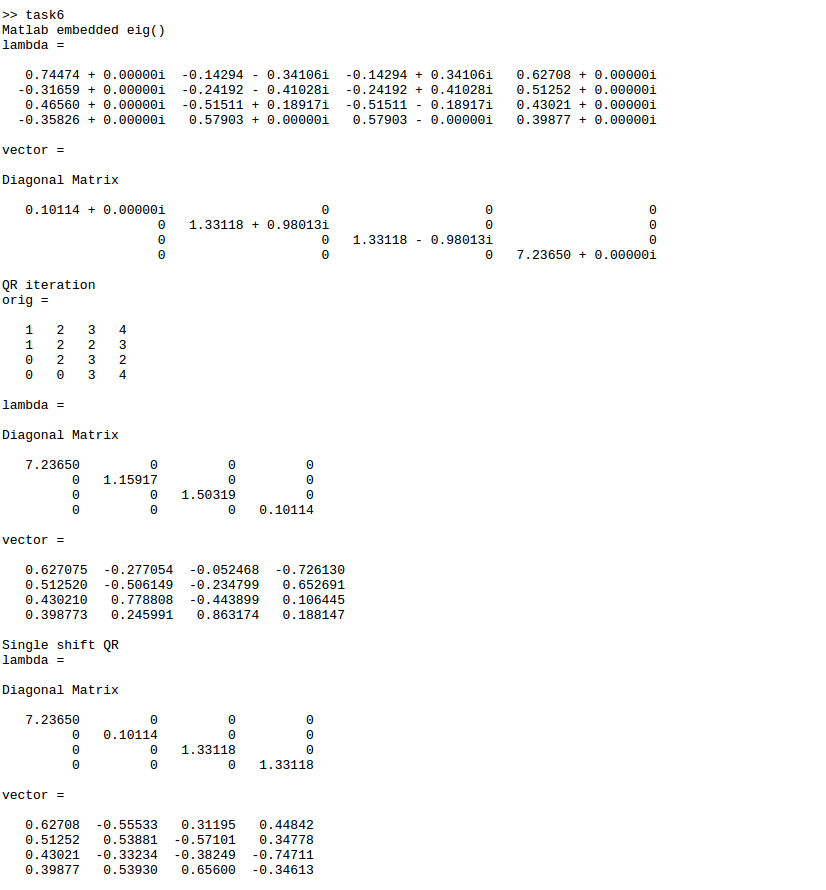
\includegraphics[width=0.7\linewidth]{screenshot008}
\label{fig:screenshot008}
\end{figure}
As the results show - the eigenvalues are all the same in case of every method that was used. According to the eigenvectors, only the dominant one match one each other.\\
It can be a matter of fact, that the solutions are iterative and only approximate.

Now, we can also perform some computations (as it was stated in previous report - each try is a 1000 round loop).
\\
\begin{lstlisting}
Matlab embedded eig()
Elapsed time is 0.016705 seconds.
QR iteration
Elapsed time is 5.19331 seconds.
Single shift QR
Elapsed time is 5.3176 seconds.
\end{lstlisting}
There is a huge difference between first algorithm (embedded) and the coded QR's. It is certainly the effect of using coded by author QR factorization.
\\
\\
Performing simple test (changing QR factoriation to matlab embedded inside coded algorithm) will show the truth. And in fact it is, as expected -- much shorter execution time:
\begin{lstlisting}
Matlab embedded eig()
Elapsed time is 0.0244899 seconds.
QR iteration
Elapsed time is 0.185272 seconds.
Single shift QR
Elapsed time is 0.28676 seconds.
\end{lstlisting}
\newpage
\textbf{Problem 7} - Draw the Gershgorin discs and determine the location of the eigenvalues for the matrices. Then compute an approximate eigensystem.
\begin{figure}[h]
\centering
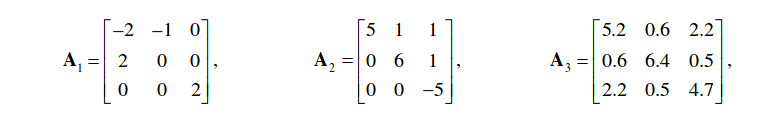
\includegraphics[width=0.7\linewidth]{screenshot009}
\label{fig:screenshot009}
\end{figure}

The Gershgorin circles are based on matrices:\\
- circles centers are indicated by the numbers on main diagonal,\\
- item circle radius is the sum of the remaining elements in the current row.\\
\begin{figure}[h]
\centering
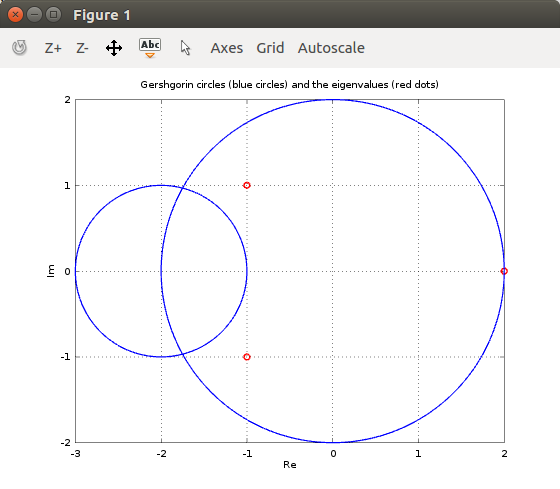
\includegraphics[width=0.5\linewidth]{screenshot010}
\label{fig:screenshot010}
\end{figure}

\begin{figure}[h]
\centering
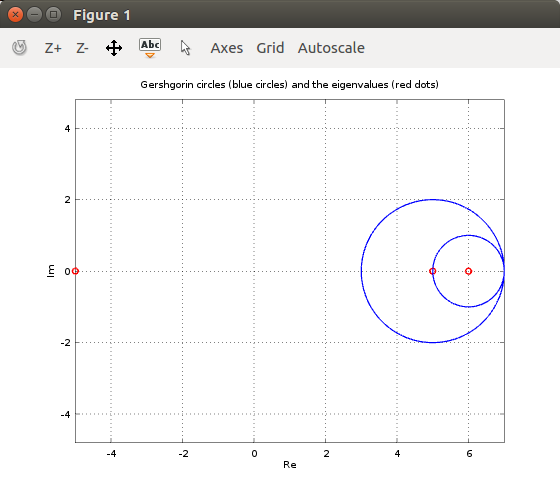
\includegraphics[width=0.5\linewidth]{screenshot011}
\caption{Matrix A1 and A2}
\label{fig:screenshot011}
\end{figure}

\begin{figure}[h]
\centering
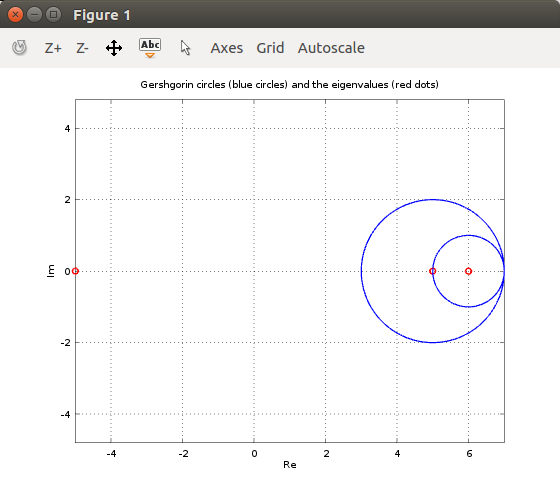
\includegraphics[width=0.7\linewidth]{screenshot012}
\caption{Matrix A3}
\label{fig:screenshot012}
\end{figure}
\newpage
As the algorithms for complex eigenvalues are currently not finished, only the real eigenvalues will be calculated.

\begin{lstlisting}
>> task7
A1 =
-2  -1   0
2   0   0
0   0   2

l =
-1.52644 -0.47356 2.00000

A2 =
5   1   1
0   6   1
0   0  -5

l =
5 6 -5

A3 =
5.20000   0.60000   2.20000
0.60000   6.40000   0.50000
2.20000   0.50000   4.70000

l =
7.6512 5.9132 2.7356
\end{lstlisting}
As compared to the visual results, for matrices A2 and A3 that have only real eigenvalues, the results are correct. However, for matrix A only one eigenvalue matches - the one that is real.
\newpage
\begin{figure}[h]
\centering
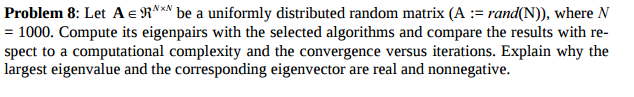
\includegraphics[width=0.8\linewidth]{screenshot013}
\label{fig:screenshot013}
\end{figure}
\begin{lstlisting}
>> task8
Coded decompositions:

Scaled power
Elapsed time is 0.00286198 seconds.

Inverse Power
Elapsed time is 0.772632 seconds.

QR
Elapsed time is 1.92643 seconds.

QR shift
Elapsed time is 1.98247 seconds.


Octave decompositions:

Eig
Elapsed time is 2.12776 seconds.

Schur
Elapsed time is 2.03479 seconds.
\end{lstlisting}

The fastest seem to be the Power methods, but we have to remember, that they calculate only the most/least dominant eigenpair, while the rest of tested algorithms calculates all the values.\\
\\
On the other hand, QR's are faster than embedded eig() or schur() function, but again: they do not resolve matrices that holds complex values.\\
The two Octave decompositions can deal with finding comples solutions (the ones that belongs to Imaginary/complex values).
\newpage
\begin{figure}[h]
\centering
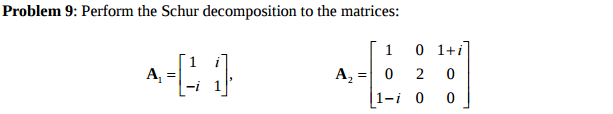
\includegraphics[width=0.8\linewidth]{screenshot017}
\label{fig:screenshot017}
\end{figure}
Schur's Triangularization results in matrix T, which on its main diagonal has the calculated eigenvalues.\\
The results of Schur decomposition were compared with Octave 'Eig()' function.
\begin{lstlisting}
>> task9
A1 Matrix Schur
U =
-0.70711 + 0.00000i  -0.70711 + 0.00000i
0.00000 + 0.70711i   0.00000 - 0.70711i

T =
2.00000  -0.00000
0.00000   0.00000


A1 Matrix embedded eig()
eigenvectors =
-0.00000 + 0.70711i   0.00000 + 0.70711i
-0.70711 + 0.00000i   0.70711 + 0.00000i

eigenvalues =
Diagonal Matrix
0   0
0   2


A2 Matrix Schur
U =
-0.81650 + 0.00000i  -0.57735 + 0.00000i   0.00000 + 0.00000i
 0.00000 + 0.00000i   0.00000 + 0.00000i   1.00000 + 0.00000i
-0.40825 + 0.40825i   0.57735 - 0.57735i   0.00000 + 0.00000i

T =
2.00000 - 0.00000i   0.00000 + 0.00000i   0.00000 + 0.00000i
0.00000 + 0.00000i  -1.00000 + 0.00000i   0.00000 - 0.00000i
0.00000 + 0.00000i   0.00000 + 0.00000i   2.00000 + 0.00000i


A2 Matrix embedded eig()
eigenvectors =
 0.40825 + 0.40825i   0.57735 + 0.57735i   0.00000 + 0.00000i
-0.00000 + 0.00000i   0.00000 + 0.00000i  -0.70711 + 0.70711i
-0.81650 + 0.00000i   0.57735 + 0.00000i   0.00000 + 0.00000i

eigenvalues =
Diagonal Matrix
-1.0000  0        0
 0       2.0000   0
 0       0        2.0000
\end{lstlisting}

\newpage
\begin{figure}[h]
\centering
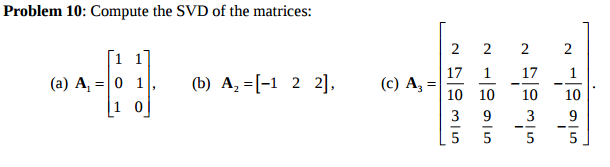
\includegraphics[width=0.8\linewidth]{screenshot014}
\label{fig:screenshot014}
\end{figure}

\begin{lstlisting}
>> task10

A1 Matrix
u =
-8.1650e-01  -7.9833e-06  -5.7735e-01
-4.0824e-01  -7.0711e-01   5.7735e-01
-4.0826e-01   7.0710e-01   5.7735e-01

s =
1.73205   0.00000
0.00001  -1.00000
0.00000   0.00000

v =
-0.70711  -0.70710
-0.70710   0.70711

A2 Matrix
u =
-0.33333   0.66667   0.66667
 0.66667   0.66667  -0.33333
 0.66667  -0.33333   0.66667

s =
3
0
0

v =  1

A3 Matrix
u =
-1.0000e+00   4.7683e-07  -2.3784e-03
-1.4274e-03  -8.0000e-01   6.0000e-01
-1.9024e-03   6.0000e-01   8.0000e-01

s =
 4.00000   0.00000   0.00000   0.00000
-0.00000  -2.00000   0.00000   0.00000
 0.00416   0.00000   3.00000   0.00000

v =
-0.50089   0.50000   0.49911  -0.50000
-0.50089  -0.50000   0.49911   0.50000
-0.49911  -0.50000  -0.50089  -0.50000
-0.49911   0.50000  -0.50089   0.50000
\end{lstlisting}

\begin{figure}[h]
\centering
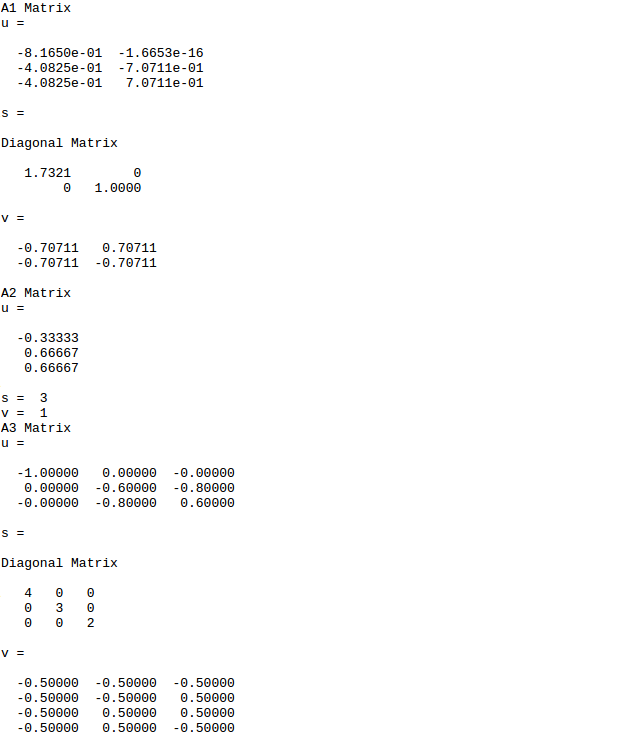
\includegraphics[width=0.7\linewidth]{screenshot015}
\caption{Embedded Octave SVD function}
\label{fig:screenshot015}
\end{figure}

As the figure \ref{fig:screenshot015} shows, the results are either very similar or identical. The SVD decomposition was coded properly. \\

As an addition to this task, the timing calculations were performed.
As usual -- the values are given regarded to 1000 rounds to avoid time needed for set-up the environment.
\begin{lstlisting}
>> task10
A1 Matrix
Elapsed time is 0.371863 seconds. (coded)
Elapsed time is 0.016098 seconds.

A2 Matrix
Elapsed time is 0.303616 seconds. (coded)
Elapsed time is 0.014389 seconds.

A3 Matrix
Elapsed time is 0.35204 seconds.  (coded)
Elapsed time is 0.0203929 seconds.
\end{lstlisting}

The embedded Octave svd is much faster, than the coded one. Even taking under consideration the fact, that coded algorithm performed only 10 iterations per round.
\newpage
\begin{figure}[h]
\centering
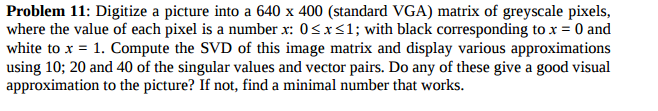
\includegraphics[width=0.8\linewidth]{screenshot016}
\label{fig:screenshot016}
\end{figure}
The following task11.m file shows the steps that were taken in order to present different compression of image using SVD decomposition.\\
(Image of resolution 640x480 was used)

\begin{lstlisting}
pkg load image # load octave package for image processing


image = imread('biedronka.jpg');	# load image
image = rgb2gray(image);			# convert to grayscale
image = im2double(image);			# process as double

iterations=100;

[u,s,v] = svd(image,iterations);

approximation=10;
image10 = u(:,1:approximation)*s(1:approximation,1:approximation)*v(:,1:approximation)';
approximation=20;
image20 = u(:,1:approximation)*s(1:approximation,1:approximation)*v(:,1:approximation)';
approximation=40;
image40 = u(:,1:approximation)*s(1:approximation,1:approximation)*v(:,1:approximation)';
approximation=80;
image80 = u(:,1:approximation)*s(1:approximation,1:approximation)*v(:,1:approximation)';

subplot(3,2,1), imshow(image),   title('Original 640x480')
subplot(3,2,3), imshow(image10), title('approximation=10')
subplot(3,2,4), imshow(image20), title('approximation=20')
subplot(3,2,5), imshow(image40), title('approximation=40')
subplot(3,2,6), imshow(image80), title('approximation=80')
\end{lstlisting}
\newpage
As the pictures below shows - using different numbers of eigenvectors results in 'image compression'. In this case, the 40 eigenvectors are enough to see a nice picture with minimal noise that does not disturb the human eye.
\begin{figure}[h]
\centering
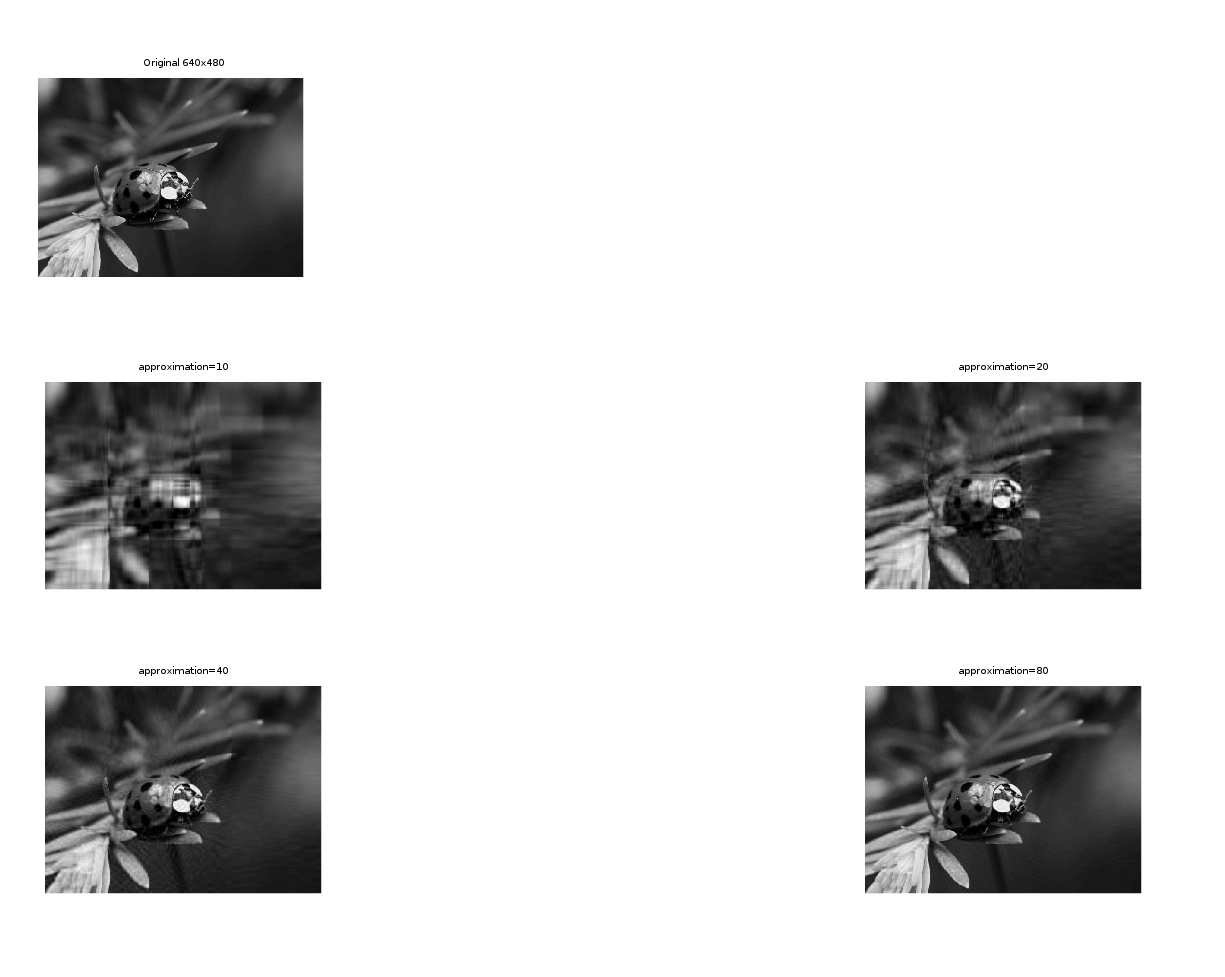
\includegraphics[width=1.1\linewidth]{screenshot018}
\caption{Results of SVD image compression.}
\label{fig:screenshot018}
\end{figure}


\chapter{Listings of algorithms}
\section{Coded selected algorithms}
Algorithm 1 - Scaled Power algorithm\\
It calculates the dominant eigenvalue and eigenvector. 
\begin{lstlisting}
function [lambda, vector] = scaledpower(A, iterations)

[n,n] = size(A);

q_prev = rand(n,1);
q_prev = q_prev/norm(q_prev);

lambda = [];
q = [];

for i = 1:iterations
z = A * q_prev;
q = z/norm(z);
q_prev = q;
endfor

#calculating Rayleigh quotient
lambda = (q'*A*q)/(q'*q);
vector = q;
endfunction
\end{lstlisting}
\newpage
Algorithm 2 - Inverse Power algorithm\\
In contrary to previous one - the result is the least significant eigenpair.
\begin{lstlisting}
function [lambda, vector] = inversepower(A, iterations)

[n,n] = size(A);

q_prev = rand(n,1);
q_prev = q_prev/norm(q_prev);
alpha = 1;
I = eye(n);
q = [];
v=[];
for i = 1:iterations

v = inv(A - alpha*I)*q_prev;
q = v/norm(v);
q_prev = q;
endfor

lambda = (q'*A*q)/(q'*q);
vector = q;

endfunction

\end{lstlisting}
Algorithm 3 - Basic QR iterations\\
Algorithm calculates the eigenvalue and eigenvectors (based on all Q product).
\begin{lstlisting}
function [lambda, vector] = iterqr(A, iterations)

[n,n] = size(A);
Qproduct = eye(n,n);

for i = 1:iterations
[Q,R] = QRgivens_lecture(A);    #calculating QR
A = R*Q;                		# assigning next step A

Qproduct = Qproduct*Q;    		# eigenvectors are product of all Qs

endfor

lambda = diag(diag(A));
vector = Qproduct;

endfunction
\end{lstlisting}
\newpage

Algorithm 4 - Shift QR algorithm\\
Algorithm calculates the eigenvalue and eigenvectors (based on all Q product).
\begin{lstlisting}
function [lambda, vector] = iterqr_shift(A, iterations)

[n,n] = size(A);

Qproduct = eye(n);
I = eye(n);


for i = 1:iterations
s = A(n,n);                       #choose the element for shift
shift = s*I;                      #create shifting diagonal

[Q,R] = QRgivens_lecture(A-shift);#apply QR factorization
A = R*Q+shift;

Qproduct = Qproduct*Q;            #multiply Q product by new Q

endfor

lambda = diag(diag(A));
vector = Qproduct;
endfunction
\end{lstlisting}

Algorithm 10 - SVD decomposition using QR.\\
Algorithm calculates the eigenvalue and eigenvectors (based on all Q product).
\begin{lstlisting}
function [U, S, V] = svdQR(A,iterations)

[n, m]= size(A); # can be rectangular matrix
U=eye(n);   
V=eye(m);

R=A';  

for i = 0:iterations
[Q,R]=qr(R');   # qr decompositions and updating  
U=U*Q;    
     
[Q,R]=qr(R');
V=V*Q;

endfor
S=R';               # S is R transposed

endfunction
\end{lstlisting}
\begin{thebibliography}{8}
\addcontentsline{toc}{chapter}{Bibliography}
%\addcontentsline{toc}{section}{Literatura}
\bibitem{bjorck}
Björck, Åke. Numerical methods for least squares problems. Society for Industrial and Applied Mathematics, 1996.
\bibitem{golub}
Golub, Gene H., and Charles F. Van Loan. "Matrix computations, 3rd." (1996).
\bibitem{zdunek}
Zdunek R., Numerical Methods - lecture slides.
\end{thebibliography}

\end{document}

